\subsection{Dataset}
\label{sec:dataset}

\begin{figure*}[htbp]
\centering
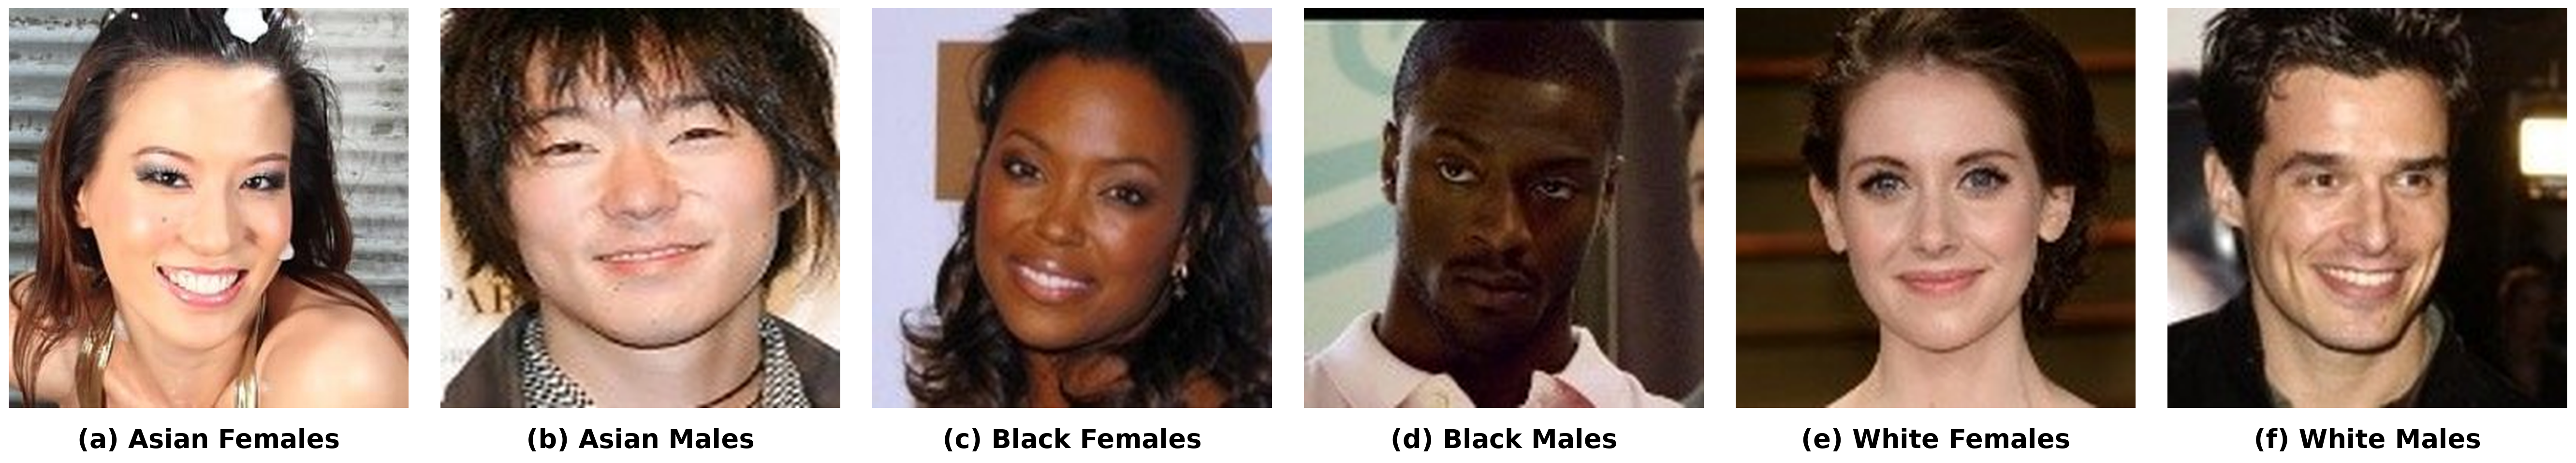
\includegraphics[width=\textwidth]{sample_demogpairs_v2.png}
\caption{Sample Images of the DemogPairs Dataset across Six Intersectional Demographic Subgroups: (a) Asian Females, (b) Asian Males, (c) Black Females, (d) Black Males, (e) White Females, and (f) White Males.}
\label{fig:2}
\end{figure*}

The experiments in this study utilize the DemogPairs dataset~\cite{ref25}, designed as a facial verification biometric benchmark to systematically evaluate the impact of demographic disparities. This corpus comprises a total of 10,800 facial images balanced across six intersectional demographic subgroups, spanning the intersection of three macro-racial categories (Asian, Black, White) and two binary gender categories (Female, Male). The dataset structure encompasses 600 unique identities, with a uniform allocation of 100 individuals per subgroup, where each identity is represented by 18 controlled images featuring variations in pose, expression, and illumination. This balanced distribution provides a controlled evaluation environment to objectively analyze cross-subgroup performance disparities without sample size distortion. Sample images are presented in Figure~\ref{fig:2}.

\begin{table*}[htbp]
\caption{DemogPairs Dataset Partition and Subject-Disjoint Demographic Subgroup Distribution.}
\label{tab:1}
\label{tab:I}
\centering
\footnotesize
\begin{tabular}{lcccccc}
\toprule
\multirow{2}{*}{Demographic Subgroup} & \multicolumn{2}{c}{Train Set} & \multicolumn{2}{c}{Test Set (Held-Out)} & \multicolumn{2}{c}{Total} \\
\cmidrule(lr){2-3} \cmidrule(lr){4-5} \cmidrule(lr){6-7}
& Subjects & Images & Subjects & Images & Subjects & Images \\
\midrule
Asian Females & 80 & 1,440 & 20 & 360 & 100 & 1,800 \\
Asian Males & 80 & 1,440 & 20 & 360 & 100 & 1,800 \\
Black Females & 80 & 1,440 & 20 & 360 & 100 & 1,800 \\
Black Males & 80 & 1,440 & 20 & 360 & 100 & 1,800 \\
White Females & 80 & 1,440 & 20 & 360 & 100 & 1,800 \\
White Males & 80 & 1,440 & 20 & 360 & 100 & 1,800 \\
\midrule
\textbf{Total} & \textbf{480} & \textbf{8,640} & \textbf{120} & \textbf{2,160} & \textbf{600} & \textbf{10,800} \\
\bottomrule
\end{tabular}
\end{table*}

To guarantee evaluation integrity and completely eliminate the risk of identity leakage (0\% leakage), this study implements a Strict Subject-Disjoint Partitioning protocol. A total of 600 unique identities are deterministically partitioned into 480 training subjects (8,640 images) and 120 held-out test subjects (2,160 images). This stratified partitioning yields a balanced allocation of 80 training subjects and 20 test subjects per subgroup, as detailed in Table~\ref{tab:1}. The test subjects are strictly independent and were never involved during model training or hyperparameter tuning. Centered facial images are converted to 3-channel Red, Green, Blue (RGB) format and resized to a resolution of 224 $\times$ 224 pixels. Pixel intensities are normalized channel-wise according to the pre-training configuration of each respective ViT checkpoint without the addition of synthetic augmentations.
